\section{基于LSTM进行汽车位置预测的GNSS位置欺骗攻击检测算法}
\subsection{模型概述}
如\ref{sec:LSTM_gaishu}所述,LSTM作为传统RNN的改进模型,可以解决长序列问题中长期依赖的问题。对于本文中所涉及到的GNSS位置欺骗检测问题,由于汽车的移动轨迹可以看作是一个有依赖关系的连续序列,因此,可以使用LSTM作为问题的解决方案。模型的检测思路为,以被欺骗前目标车辆的CAN速度、IMU前向加速度以及转向角作为输入,输出为下一时刻目标车辆所处位置与当前车辆位置之间距离的预测值$dis_p$。计算$dis_p$与车辆实际移动距离$dis_g$的绝对值$dis_{abs}$,并设置欺骗阈值$\gamma$。若满足$dis_{abs}>\gamma$,则认为此时目标车辆受到了GNSS位置欺骗。$\gamma$的定义如下:
\begin{equation}
    \gamma=\epsilon_{GNSS}+\epsilon_{LSTM}
    \label{eq:gamma}
\end{equation}
其中,$\epsilon_{GNSS}$表示汽车GNSS模块定位误差,$\epsilon_{LSTM}$表示检测模型的预测误差。
本文所使用的模型结构包括输入层、包含50个神经元的隐藏层以及输出层。如图\ref{fig:my_model_arch}所示。
\begin{figure}[htbp]
    \begin{center}
        \includegraphics[width=0.8\textwidth]{LSTM.eps}
    \end{center}
    \caption{本文所使用的LSTM模型结构}
    \label{fig:my_model_arch}
\end{figure}

\subsection{模型训练}
\label{sec:model_train}
本文在模型训练过程中将学习率设置为0.01,batch size设置为64,并使用Adam优化器。另外,使用平均绝对误差(Mean Absolute Error,MAE)作为损失函数。MAE的定义如公式(\ref{eq:MAE})所示。
\begin{equation}
    MAE=\frac{1}{N}\sum_{i=1}^N|y_p-y_g|
    \label{eq:MAE}
\end{equation}
其中,$N$表示总样本数目,$y_p$与$y_g$分别表示模型预测距离以及真实距离。模型训练过程中模型在训练集以及测试集的损失变化情况如图\ref{fig:train_MAE_loss}所示。
\begin{figure}[htbp]
    \begin{center}
        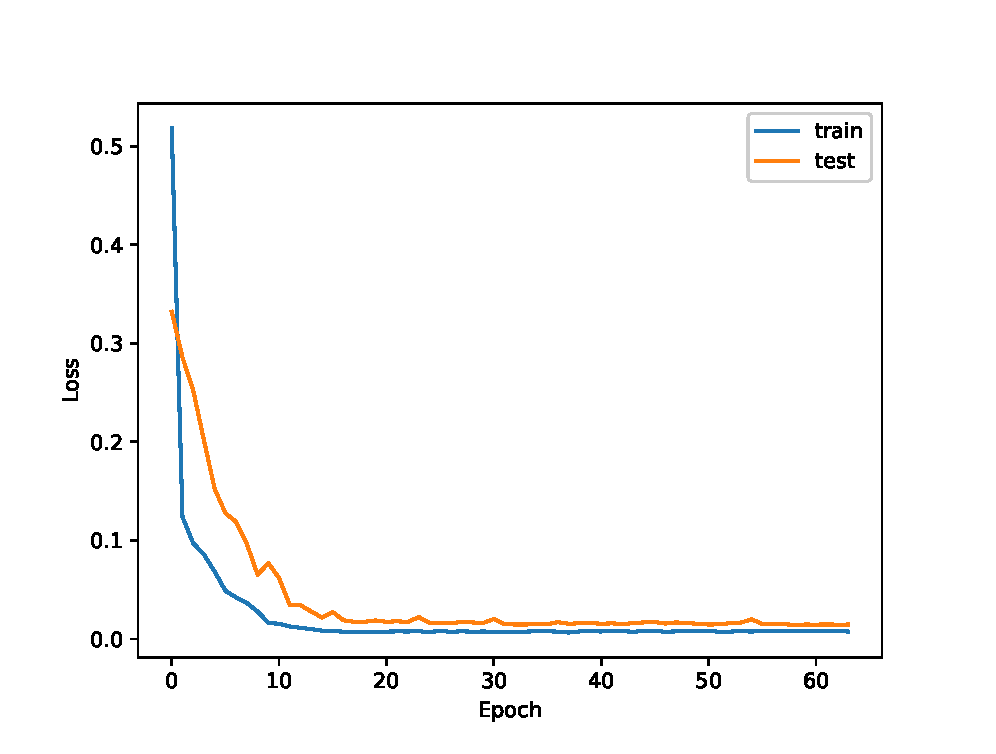
\includegraphics[width=0.8\textwidth,trim={0 10 0 10},clip]{train_loss.eps}
    \end{center}
    \caption{平均绝对误差(MAE)}
    \label{fig:train_MAE_loss}
\end{figure}

紧接着,在模型训练完成后,以RMSE作为评价指标,并统计模型的最大误差、最小误差与平均误差,从而对模型的有效性进行评估。RMSE计算公式如(\ref{eq:RMSE})所示。
\begin{equation}
    RMSE=\frac{1}{N}\sqrt{\sum_{i=1}^N(y_p-y_g)^2}
    \label{eq:RMSE}
\end{equation}
其中,$N$表示总测试样本数目,$y_p$与$y_g$分别表示模型输出的预测距离与真实距离。所得出的评估结果如表(\ref{tab:metrics})所示。

\begin{table}
    \begin{center}
    \begin{tabular}{ccl}
        \toprule
        评估指标 & 值 \\
        \midrule
        RMSE & 0.072 \\
        min error & -0.000957(m) \\
        max error & 1.043058(m) \\
        average error & 0.070112(m) \\
        \bottomrule
    \end{tabular}
    \end{center}
    \caption{模型测试后统计得出的各评估指标}
    \label{tab:metrics}
\end{table}

另外,为了直观呈现模型的有效性,图\ref{fig:model_eval}展示了测试集上预测距离值与真实距离值的曲线图。
\begin{figure}[htbp]
    \begin{center}
        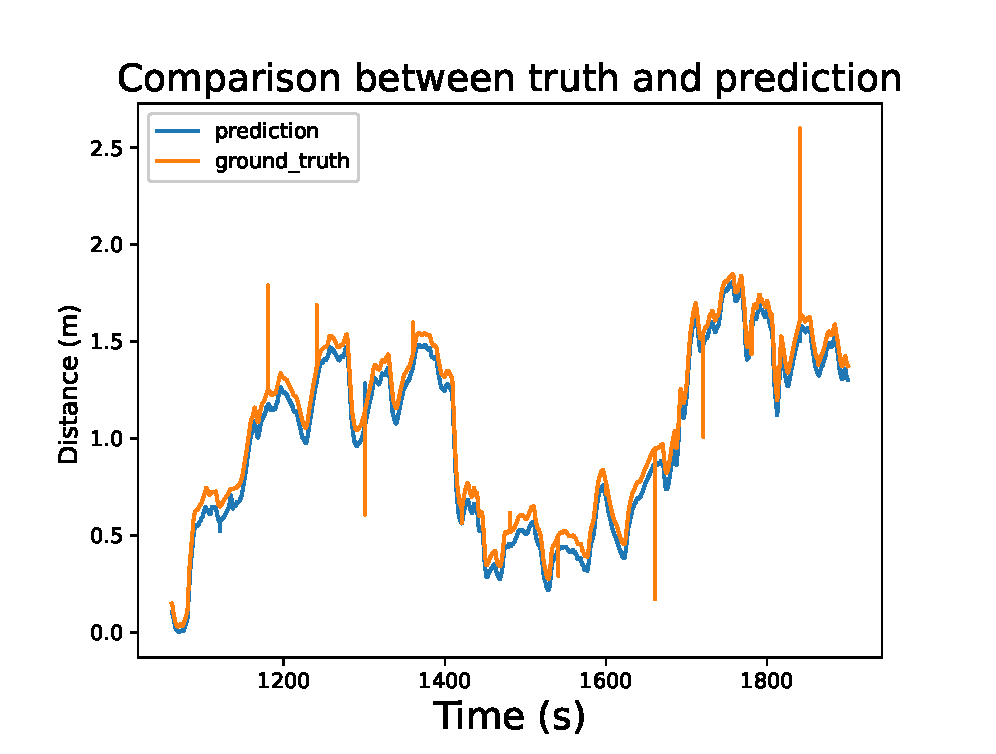
\includegraphics[width=0.8\textwidth,trim={0 0 10 0},clip]{model_eval.eps}
    \end{center}
    \caption{预测距离值与真实距离值对比}
    \label{fig:model_eval}
\end{figure}
% \zhlipsum
从表(\ref{tab:metrics})以及图\ref{fig:model_eval}可以看出,模型的预测精确度较高,可以较好地实现GNSS位置欺骗攻击检测的目的。

\subsection{GNSS位置欺骗攻击检测}
本文所采取的欺骗攻击检测方法,是通过比对上述模型的预测行驶距离与实际行驶距离来实现的。若两者间的差值大于误差阈值,则认为此时目标车辆受到了欺骗。检测算法伪代码见算法\ref{algo:dectection}。\ref{sec:model_train}中定义欺骗阈值$\gamma=\epsilon_{GNSS}+\epsilon_{LSTM}$。另外,由\ref{sec:model_train}可得知,模型的平均预测误差为0.070112m;同时,由\cite{kaplan2005understanding}可知,目前常用的GNSS定位技术误差可认为是10m。因此,有$\gamma=10+0.070112(m)$。

\begin{algorithm}
    \KwIn{来自CAN的车速$v$, 来自IMU的前向加速度$a_{forward}$, 转向角$\omega$,来自GNSS模块的实际行驶距离$dis_{truth}$,行驶距离预测模型$M$,欺骗阈值$\gamma$}
    \KwOut{表示是否受到欺骗的布尔值$spoofed$}
    $dis_{predict}=M(v, a_{forward}, \omega)$\;
    \eIf {$\|dis_{predict}-dis_{truth}\|>\gamma$}
    {
        $spoofed\leftarrow True$\;
    }{
        $spoofed\leftarrow False$\;
    }
    \KwRet{$spoofed$}\;
    \caption{GNSS位置欺骗攻击检测算法}
    \label{algo:dectection}
\end{algorithm}

\subsection{本章小结}
本章主要介绍了基于LSTM的智能网联汽车GNSS位置欺骗攻击检测算法的基本思路、模型结构以及训练细节。同时通过MAE与RMSE说明了模型的有效性。
